\documentclass[11pt,oneside,english]{article}
\usepackage{geometry}
\geometry{letterpaper}
\usepackage{amssymb}
\usepackage{amsmath}
\usepackage{amsthm}
\usepackage{babel}
\usepackage{graphicx}
\usepackage{caption}
\usepackage{subcaption}
\usepackage{wrapfig}
\usepackage[parfill]{parskip}

\begin{document}

\title{Hackulus Thriftus: A New Virtual Reality}
%\subtitle{3D Reconstruction and Computer Vision Final Project}
\author{Siena McFetridge (scm2539) \\ \texttt{scmcfetridge@utexas.edu}
  \and
  Paige Hinkle (ph7457) \\ \texttt{phinkle@utexas.edu}
  \and
  Jon Lee (cjl2443) \\ \texttt{chencjlee@gmail.com}
  \and
  Jaime Rivera (rjr2426) \\ \texttt{jaimerivera@utexas.edu}
  \and
  Rohan Ramchand (rsr898) \\ \texttt{rohan@ramchand.me}}

\maketitle

\section{Overview}

The goal of virtual reality is to immerse the user in a world that, although
totally artificial, resembles the real world to a degree at which the user would
be incapable of distinguishing simulation from reality. The goal of computer
vision is to take real-world objects and situations, and translate it into terms
a computer would recognize. While the goals of each of these fields often
diverge wildly, there is one fundamental goal these two worlds share: to
virtualize, so to speak, reality.

Our project therefore attempts to bridge these worlds in a novel way. Existing
works have demonstrated that is possible to record the real world in a way
that a computer might be able to recreate it; it is only fitting that these
recreations might serve as a model for the degree of accuracy virtual reality
hopes to emulate. To that end, the goal of the Hackulus Thriftus project is to
combine the model of reality a Kinect is capable of recording with the model
of reality Google Cardboard is capable of producing.

We demonstrate a novel usage of existing mathematical techniques for
capturing a 3D model from stereoscopic camera data. We further demonstrate
an application of this data to the model of virtual reality in Google
Cardboard. We conclude with some general remarks about the results (and
quality thereof) of our project.

\subsection{Objectives and Key Results}

We divided the project into three objectives, categorized alongside key results
expected by the completion of each objective (OKRs):

\begin{description}
  \item[Objective 1]{Completion of the mapping of Kinect depth maps to point
      clouds for rotated objects}
  \item[Objective 2]{Completion of the mapping of Kinect depth maps to point
      clouds for scenes, where the Kinect is instead rotated}
  \item[Objective 3]{Completion of the translation protocol between point clouds
      and viewable scenes in Google Cardboard}
\end{description}

\section{Background}

Three-dimensional object reconstruction is a cutting edge area of computer
vision, and is currently being actively researched and developed for consumer
use. The Kinect, an accessory to Microsoft's popular Xbox 360 gaming console,
is a significant step forward in consumer-accessible 3D reconstruction
hardware, as it mimics the functionality of cutting-edge research technology.
Research has already been undertaken by Microsoft in the area of scene
creation, resulting in a proprietary library called Kinect Fusion (which has
an open-source counterpart, KinFu). Although we considered using these
libraries, OpenCV proved to be sufficient for the creation of 3D meshes.

Virtual reality has long been an active area of research and is now a popular
area of consumer technology as well, made accessible by the Oculus Rift and
Google Cardboard. The applications for virtual reality remain as of yet
untapped, but virtual reality most usefully allows for immersion into 3D
spaces. Cutting-edge technology in the virtual reality space includes modeling
and interaction with 3D objects and consumer products, such as in video games
and interactive scenes. Google Cardboard, in particular, allows for a
web-facing client that is powered by WebGL, a Javascript graphics library,
through three.js, a Javascript mesh loader.

\section{Methods}

\subsection{Kinect}

The Kinect is a motion sensing input device made by Microsoft for their line of
gaming consoles, the Xbox. It is a combination of 3 parts: a regular color
camera, an IR camera, and an IR projector. From our basic understanding, the IR
projector projects a known speckle pattern which the IR camera picks up on and
can calculate depth by figuring out the spacing of the speckles. We chose the
Kinect as our method of scanning objects because of the accuracy of the depth
maps produced, and because one was readily available and was well-supported in
OpenCV.

\begin{figure}
  \centering
  \begin{subfigure}[b]{0.45\textwidth}
    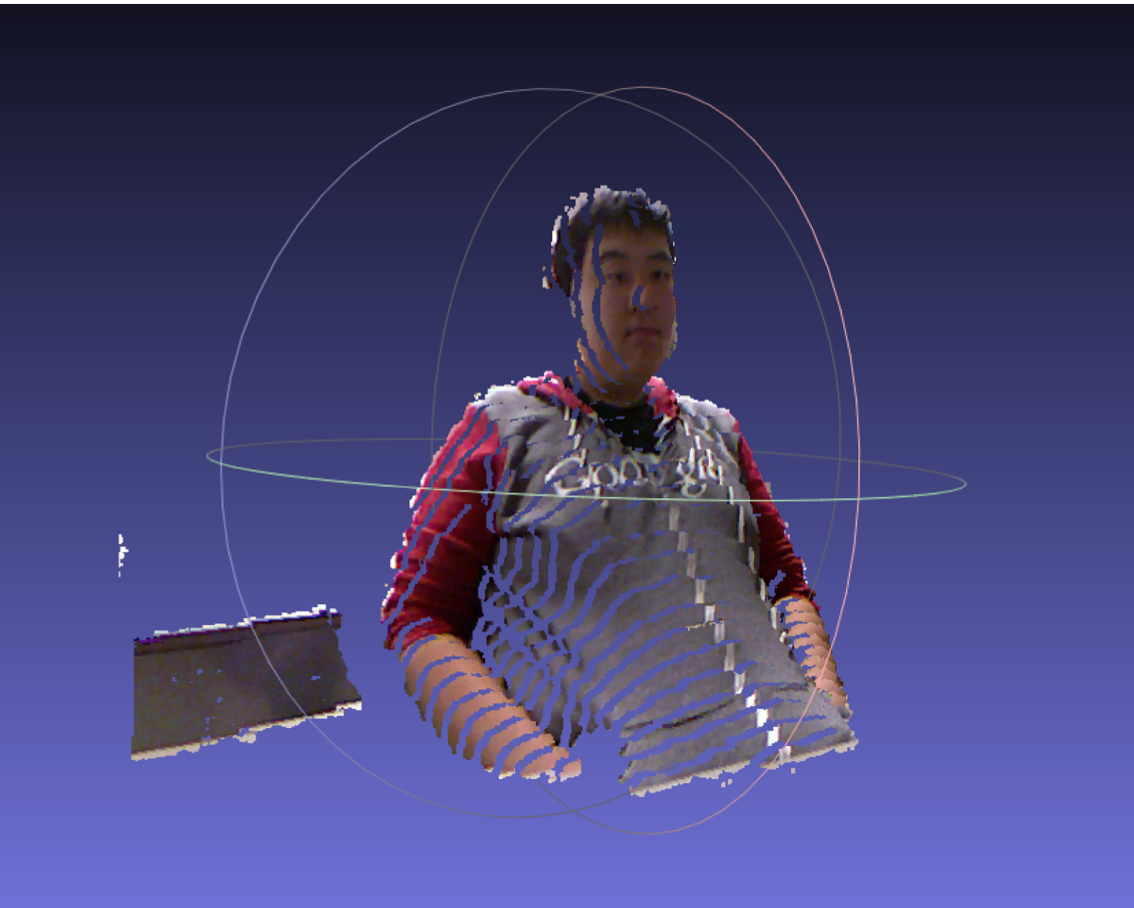
\includegraphics[width=0.9\textwidth]{jon1}
    \caption{Point-Cloud Capture}
    \label{fig:awesome_image}
  \end{subfigure}
  \begin{subfigure}[b]{0.45\textwidth}
    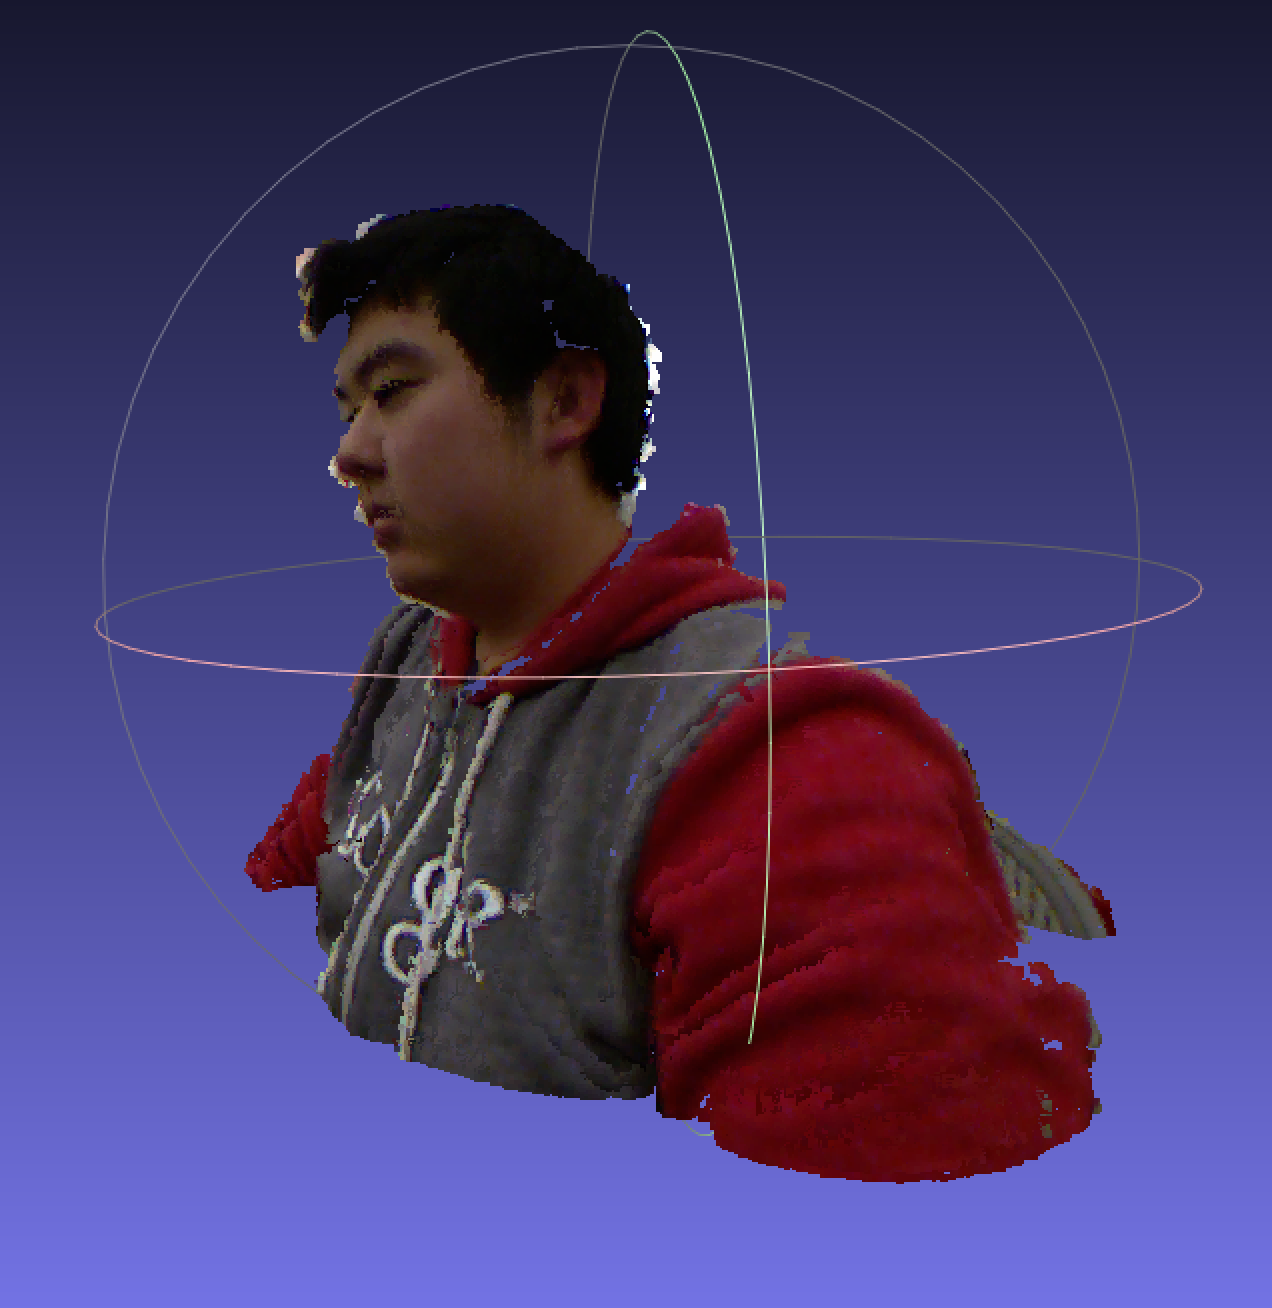
\includegraphics[width=0.8\textwidth]{jon2}
    \caption{Different Angle}
    \label{fig:awesome_image}
  \end{subfigure}
\end{figure}

Using the OpenNI library, PrimeSense's NiTE middleware, and SensorKinect
library, we were able to connect to the Kinect successfully through OpenCV.
Initially, we grabbed the disparity image and the BGR image for each frame from
the Kinect, which we ran through Project 2's disparity-to-point cloud generator.
This produced the results seen in our second progress report. Ultimately, we
felt that the point clouds generated in this fashion were not very detailed, in
that the depths were discontinuous. In searching for a better method, we found
that we could get the raw depth map from the Kinect in millimeters from each
pixel. Combining this with the BGR information from the color camera, we were
able to generate a much better point cloud, as seen above.

Since we were now able to construct detailed 3-dimensional point clouds from the
Kinect, the next objective to tackle was to properly transform different point
clouds onto one another. To simplify the problem, we believed that a single
object on a lazy susan would be ideal, since we would only need to solve for the
center of rotation and rotation matrix. We took each image from the Kinect and
found corresponding features between the images. These were the points within
the point cloud that we used to find the optimal rotation. We toyed with the
idea of using a clever ternary search algorithm to eliminate having to manually
rotate the object by specific degrees.

\begin{wrapfigure}{r}{0.5\textwidth}
  \begin{center}
    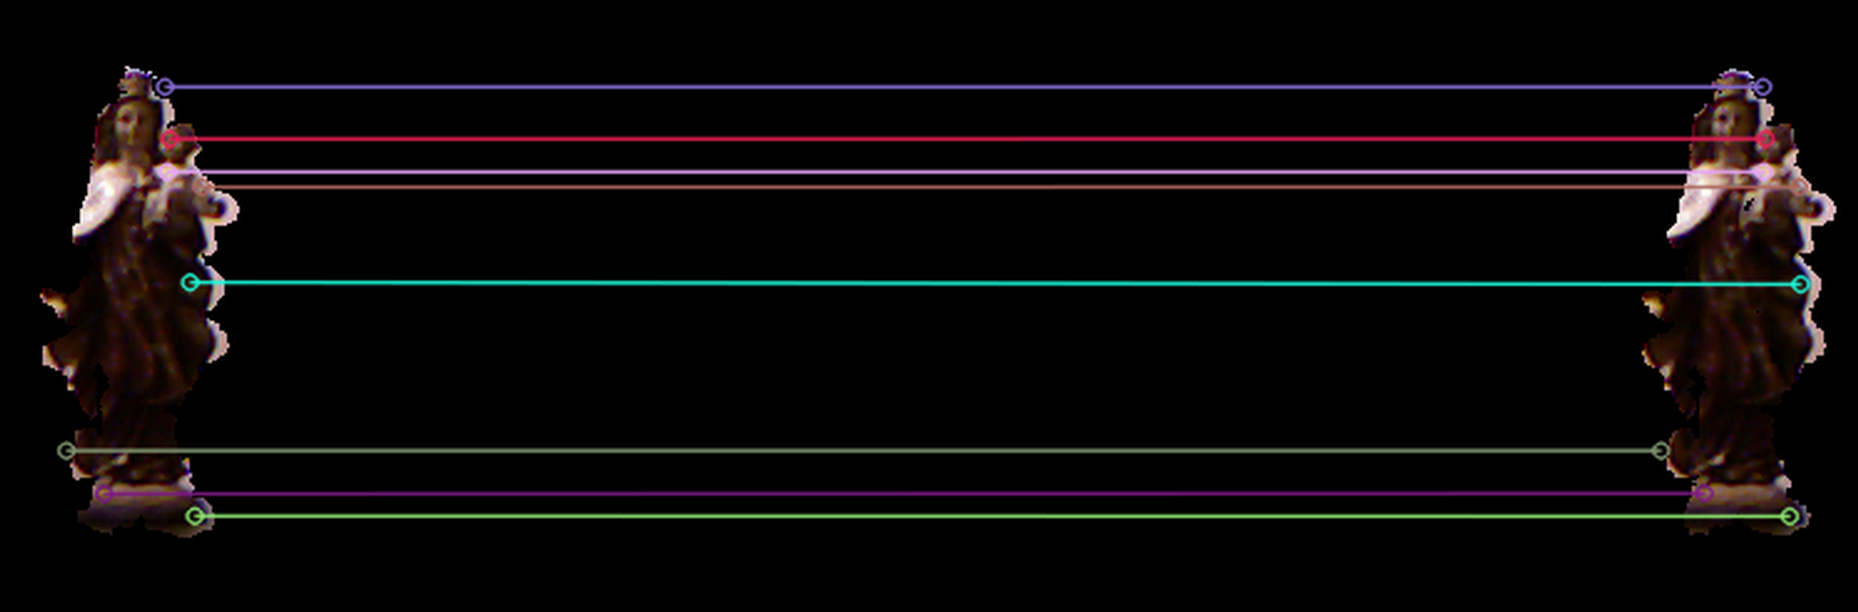
\includegraphics[width=0.48\textwidth]{feature}
  \end{center}
  \caption{Feature Matching in OpenCV}
\end{wrapfigure}

However, as this approach would have made an unreasonable amount of assumptions
about the environment, we decided to feature match as usual, but to use Singular
Value Decomposition (SVD) to find the rigid transform between the two point
clouds; in particular, we relied primarily on the SVD implementation supplied by
OpenCV. The main issue was therefore reduced to proper feature matching between
the images. We found features using SURF, created descriptors from SIFT, and
finally matched using a brute force matcher. To reject further points, we made
the assumption that our rotation was along the y-axis, which simplified the
problem without making unreasonable or incorrect assumptions. The issue remains
that the Kinect base needs to be perpendicular to the axis of rotation of the
object. We believe this approach should work fairly well, but we were unable to
properly apply our matrix transformations.

\begin{wrapfigure}{l}{0.7\textwidth}
  \begin{center}
    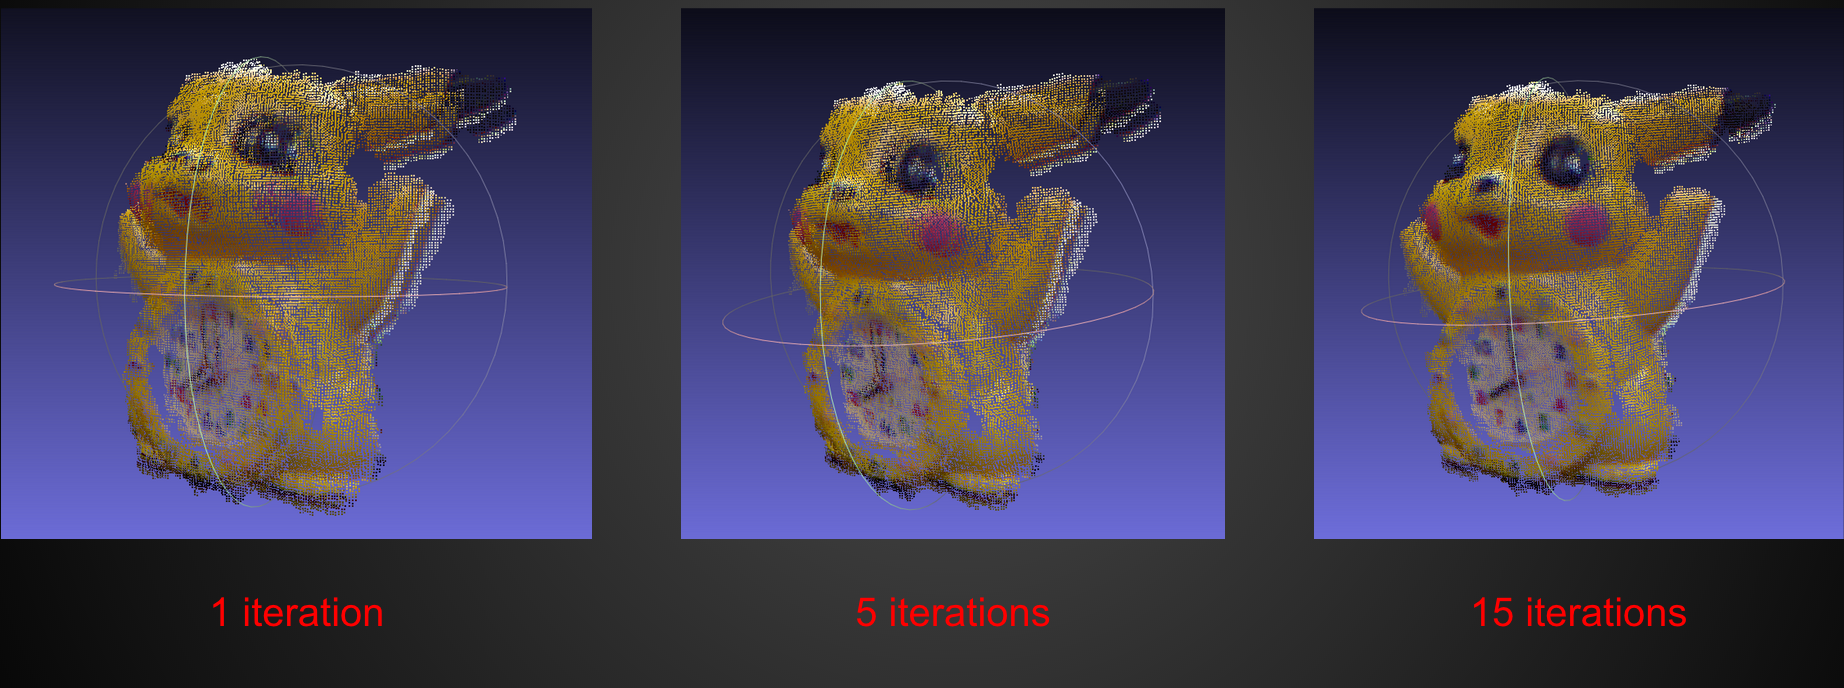
\includegraphics[width=0.68\textwidth]{pika3}
  \end{center}
  \caption{Quality over Iterations}
\end{wrapfigure}

Frustrated, we started working on a new implementation of our current work, this
time more carefully implementing the interactions with OpenCV's Mat matrix
format. In the process, we also decided to fully implement Iterative Closest
Point (ICP). ICP is one of the current industry standards for point cloud
registration. The way it works is by finding the nearest neighbor in the
registered points for each point to be registered and calculating an optimal
transformation matrix to transform the points to their neighbors that minimizes
error. After transforming the registrant points, the process is repeated again,
multiple times, with each iteration getting closer and closer to a good match.
ICP requires a set of correspondences, much like our previous implementation.
This time we opted out of using the feature detection to find correspondences
because of small issues we had, and instead took the entire point cloud union as
we iterated and found the closest points, using OpenCV's Flann index KD tree, to
the new point cloud to be registered, as our correspondent points. Due to the
nature of ICP, implementations usually require some initial guess of the spatial
orientation of the point cloud to be registered. To avoid using an algorithm
like PCA, we instead rotated the entire union of point clouds registered so far,
so that the point cloud to be registered and the union of point clouds were
fairly close to start off with from the view of the Kinect’s frames.

This approach ran very slowly, but we were able to overcome this by instead
accumulating the rotation and translation matrices from previous registrations
and applying that to the registrant point cloud. We then further optimized the
registration process, by using a random sampling of points between each frame,
and using those for the initial set of correspondences, instead of the entire
point cloud. This increased efficiency by an order of magnitude, and allowed us
to generate significantly larger sets using many more points. We believe that
employing feature matching into the picture to have an initial set of
correspondences that are closer than the rotation of the entire point cloud
would also positively affect efficiency, but we did not further explore the
idea.

\subsection{Cardboard}

We decided to use Google Cardboard for our virtual reality viewer because the
learning curve is significantly shallower than the more complicated Oculus Rift.
Instead of Unity, the framework that powers the Rift, Cardboard supports a
JavaScript-based web application or an Android application. We chose to make a
web application to view our 3D scans created using the Kinect.

The harness for the initial setup is supplied by Google for developers. It
splits the screen in half with a slight offset to create the optical 3D
illusion. This is created using Javascript, WebGL and three.js. Making a virtual
reality scene does not differ from creating a 3D graphic scene after splitting
the views, and so therefore to create the scene, we added a modified camera,
additional lighting, and a 3D representation of our Kinect scans. This 3D object
was created by loading in our scan and converting it into a WebGL object. 

We decided to create an object (.obj) file from the 3D scans we were expecting
as output from the Kinect to make loading the imagery into Cardboard via
three.js simple, as open-source loaders already existed. However, we instead
were forced to write a point cloud (.ply) loader from scratch, as no open-source
alternative existed for JavaScript. This involved parsing each line in the file,
which contained a point's coordinates and RGB values. The points required some
fine tuning to suit the three.js format, and then were added to a Geometry
object which contained all the points. The RGB values were saved in a Color
object, and then associated with the Geometry object at the end. This could then
be converted to an object and material which could then be added to the scene.

\section{Results}

\subsection{Kinect}

\begin{figure}[h]
  \centering
  \begin{subfigure}[b]{0.45\textwidth}
    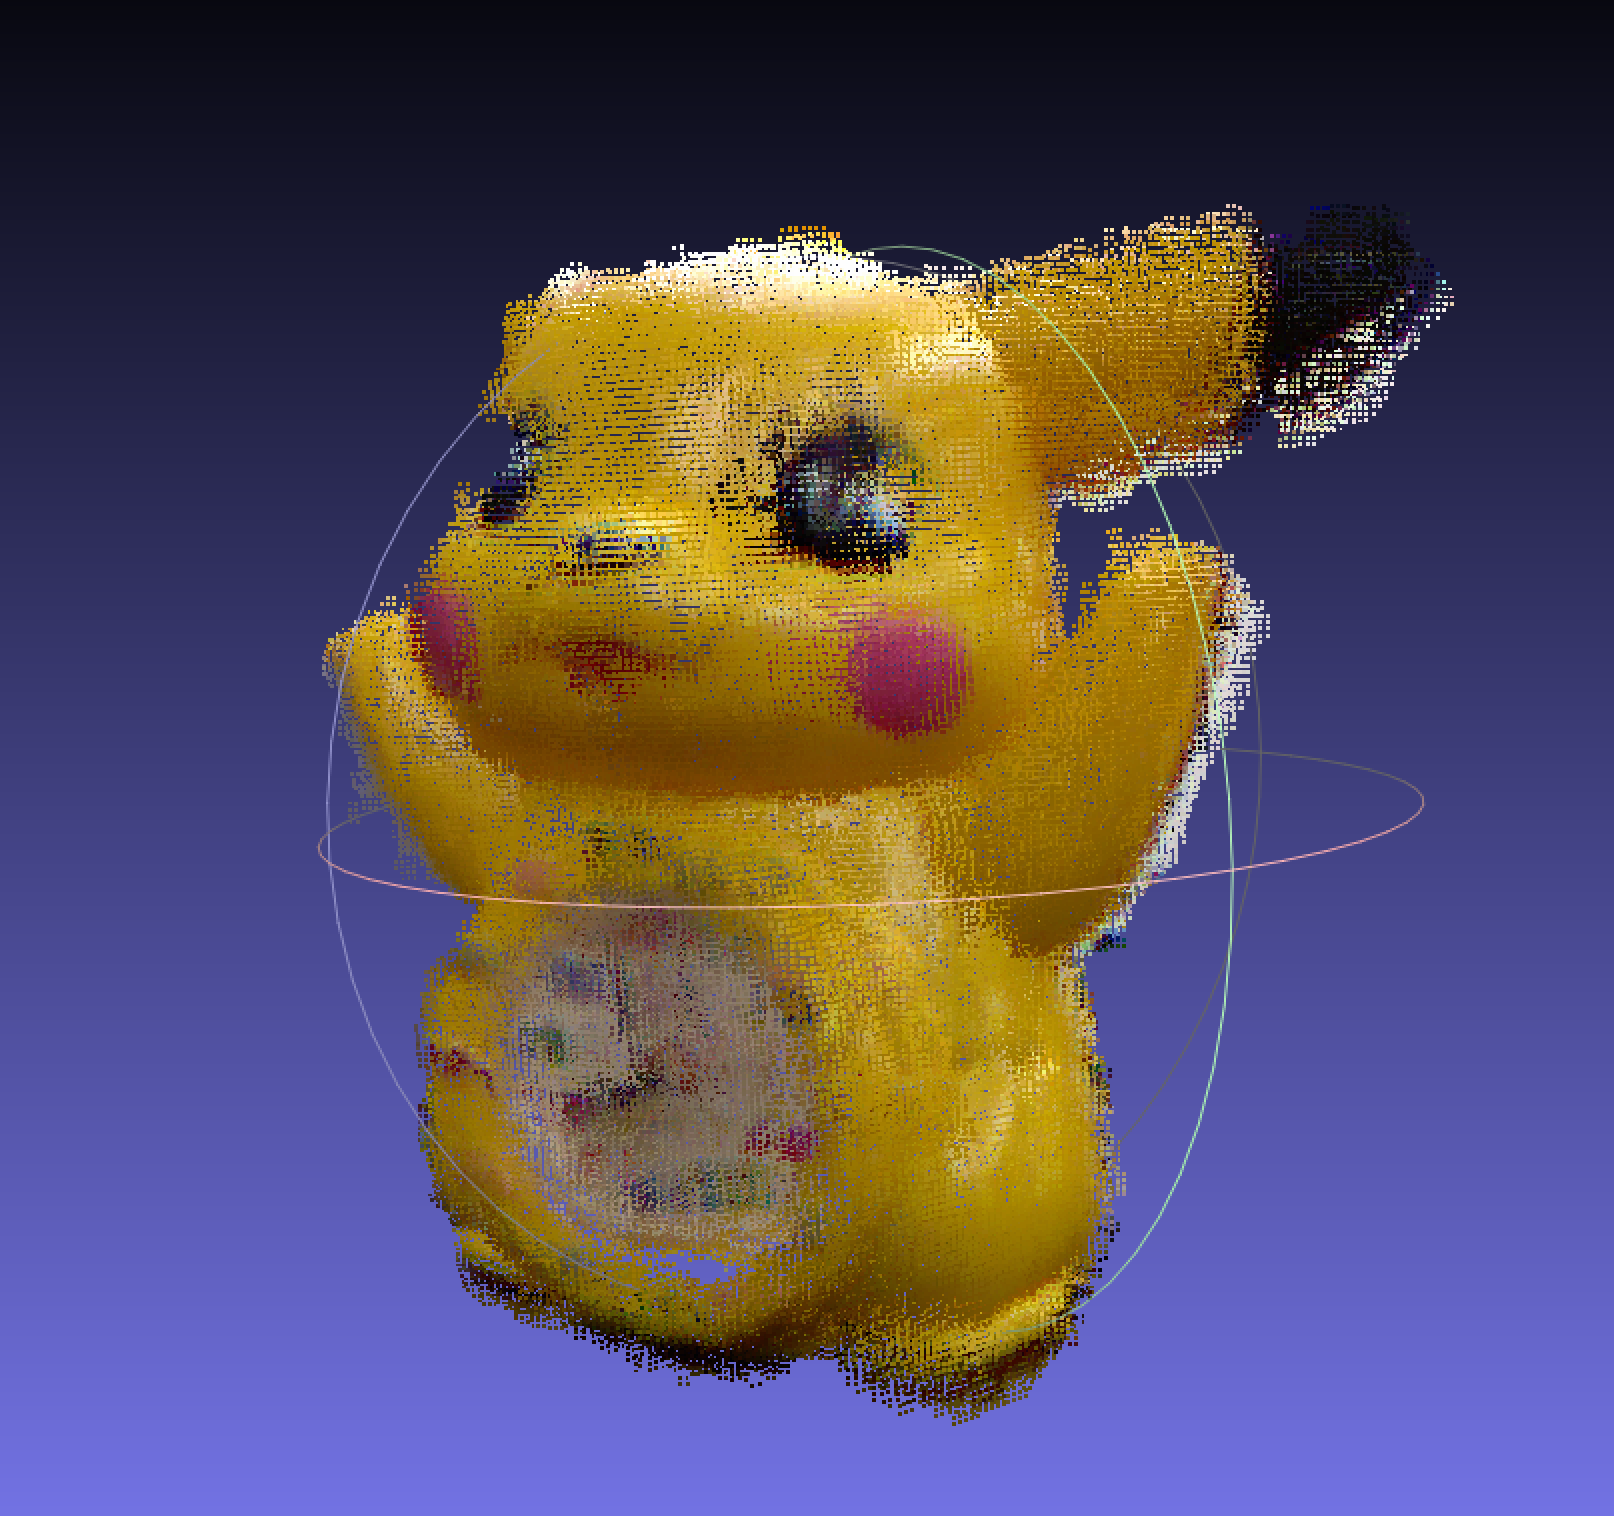
\includegraphics[width=0.9\textwidth]{pika1}
    \caption{Final Point-Cloud Capture}
    \label{fig:awesome_image}
  \end{subfigure}
  \begin{subfigure}[b]{0.45\textwidth}
    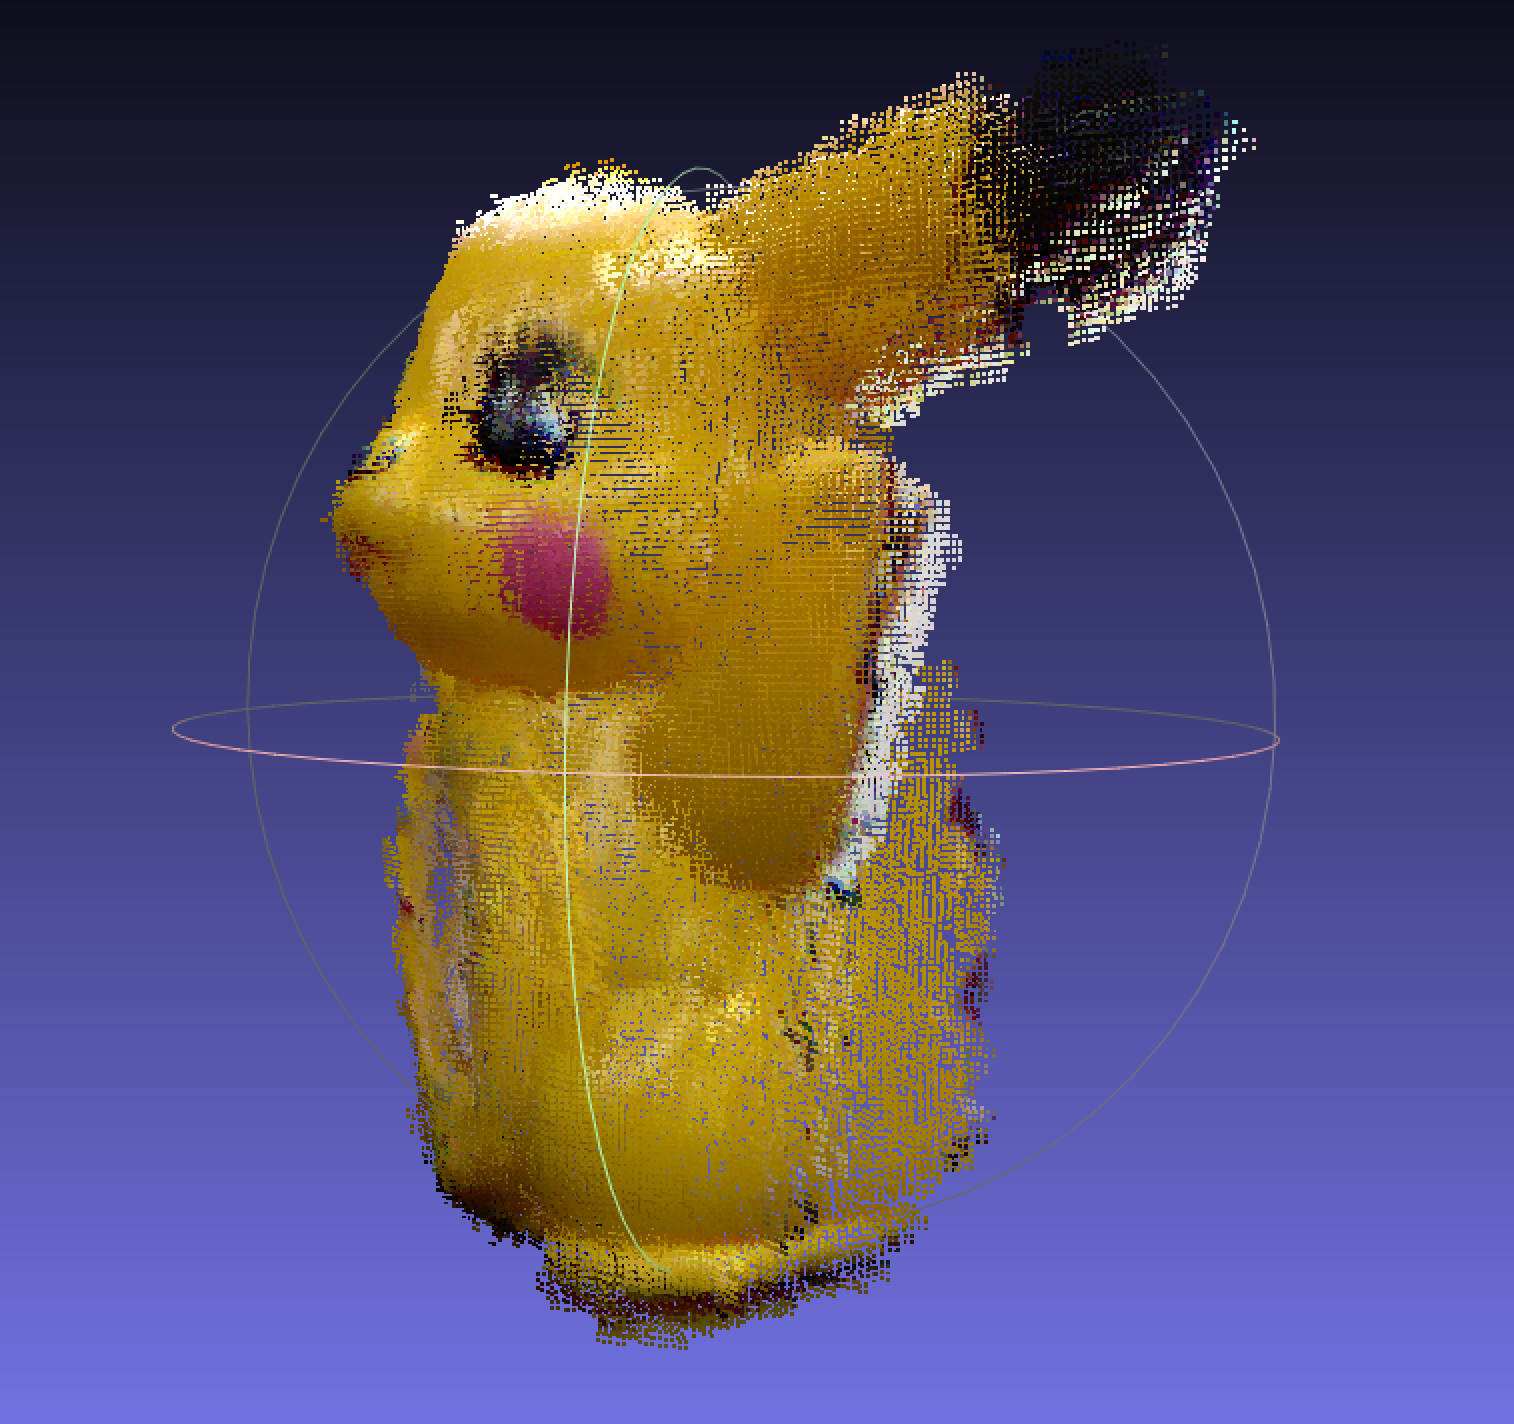
\includegraphics[width=0.8\textwidth]{pika2}
    \caption{Different Angle}
    \label{fig:awesome_image}
  \end{subfigure}
  \begin{subfigure}[b]{0.45\textwidth}
    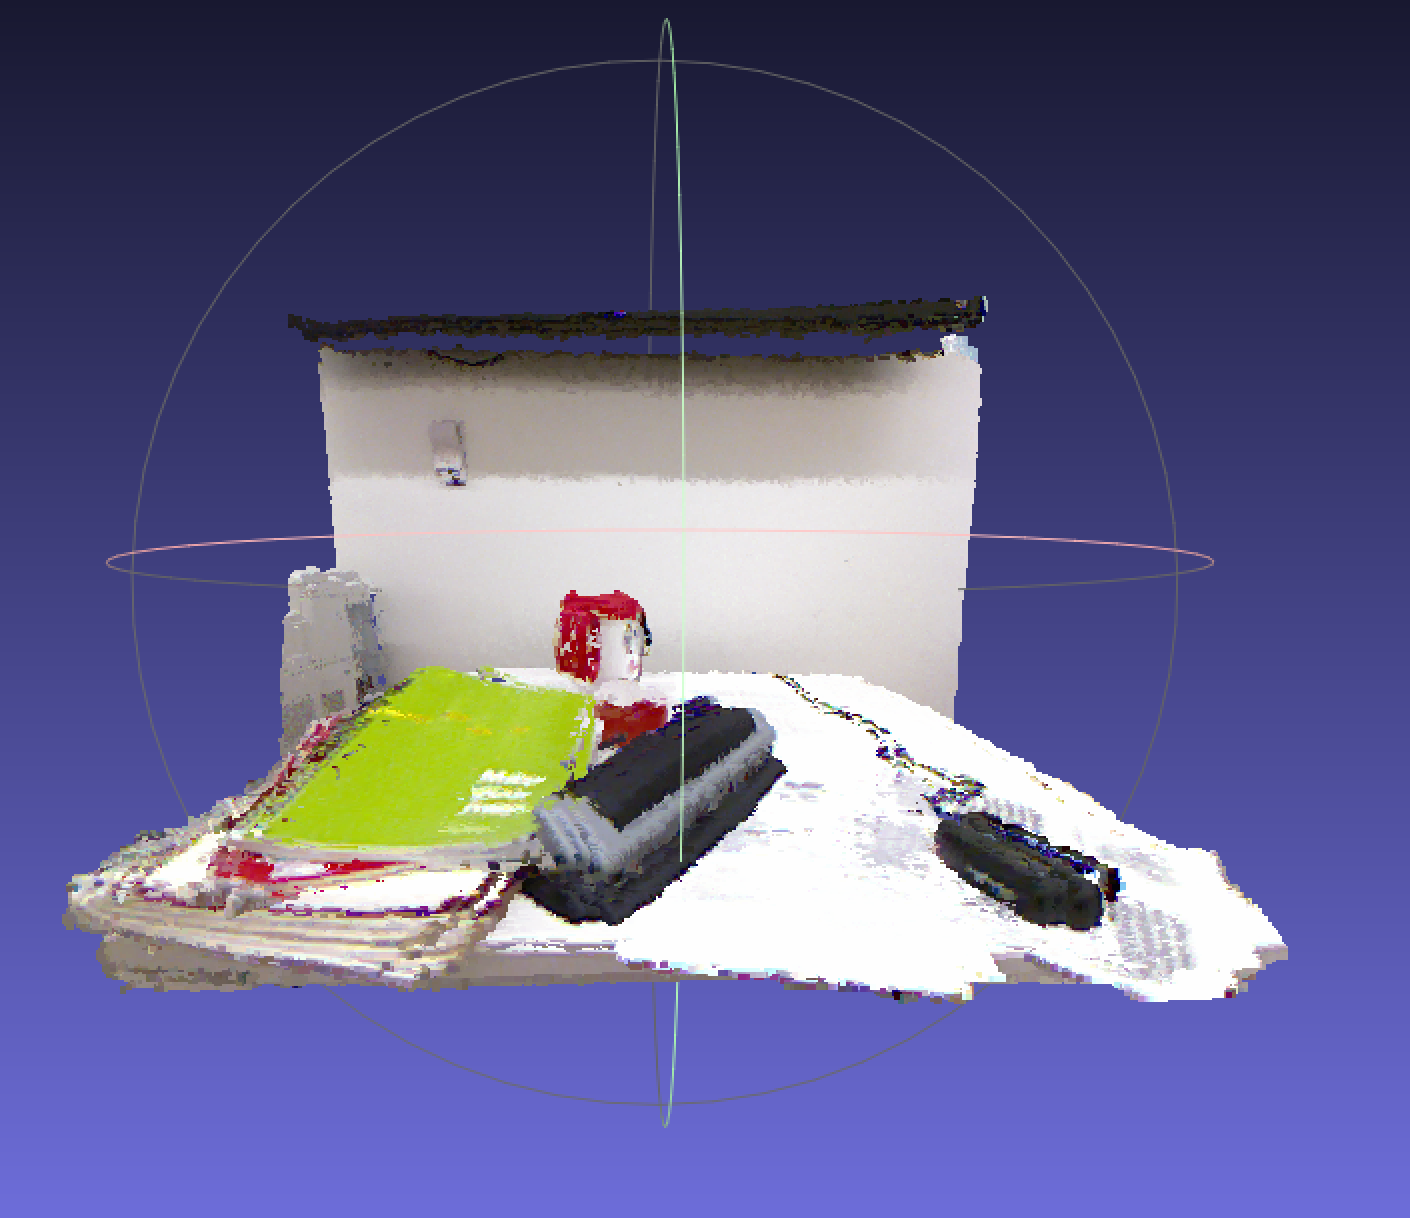
\includegraphics[width=0.9\textwidth]{desk1}
    \caption{Final Point-Cloud Capture}
    \label{fig:awesome_image}
  \end{subfigure}
  \begin{subfigure}[b]{0.45\textwidth}
    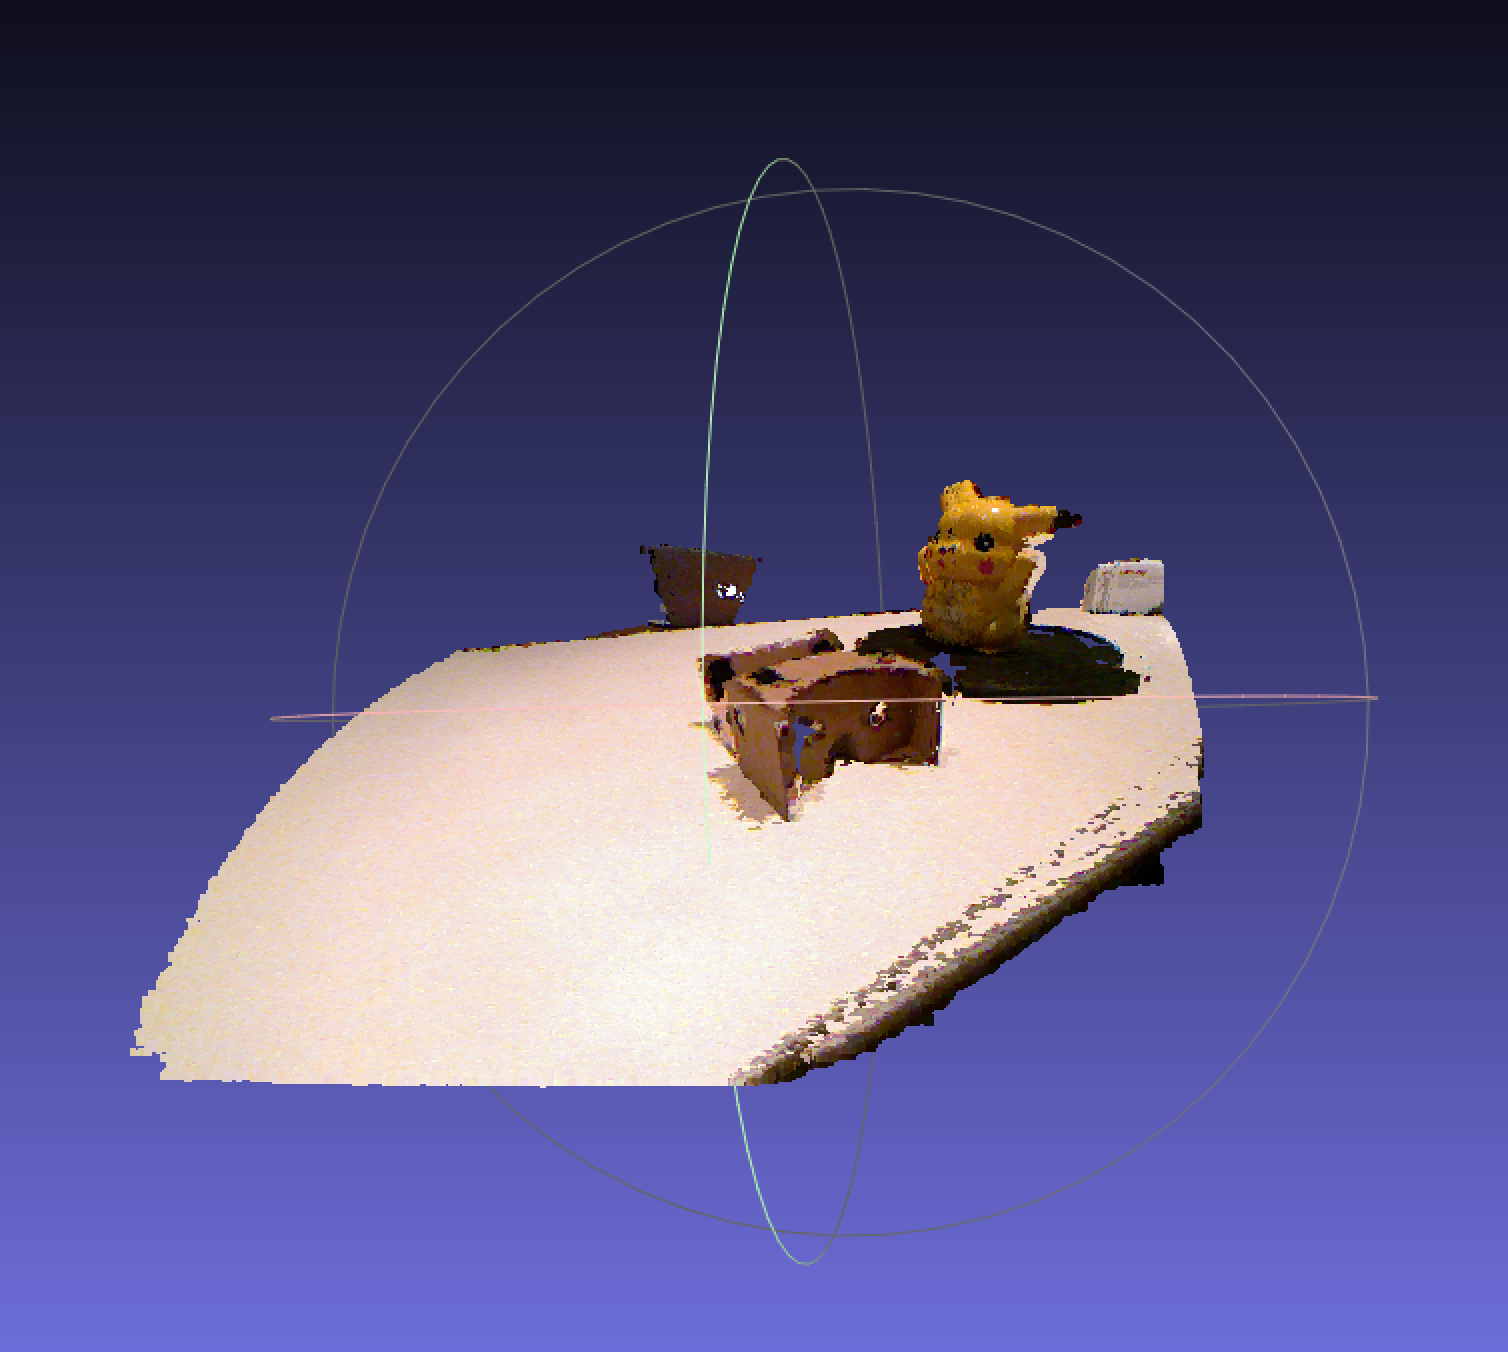
\includegraphics[width=0.8\textwidth]{desk2}
    \caption{Different Angle}
    \label{fig:awesome_image}
  \end{subfigure}
\end{figure}

For the Kinect portion of the project, we initially set two major goals: to
recreate a 3D object by moving an object in front of the Kinect and to recreate
a 3D scene by moving the Kinect. We were able to complete both goals by
re-creating both a Pikachu alarm clock and by re-creating the table next to the
GDC 3rd Floor Lab Printer.

While we achieved the intent of both our original goals, we did not fully
complete them, due to irrelevance of the initial goal or due to technical
difficulties. Our original goal for scanning a scene using a rotating Kinect
became irrelevant because we were able to scan a scene by fully moving the
Kinect around. On the other hand, because of the complexity we didn't expect in
implementing the point cloud registration algorithm, we decided to put creating
meshes out of our point clouds on the back burner. This ended up not being
detrimental to the spirit of our project though, because we were able to
implement viewing of point clouds in Cardboard.

There were also some limitations to our solutions. Our current implementation is
unable to generate a full 360-degree model of an object, often times failing
after about a 90-120 degree rotation; we believe this is due to a bug in our
implementation with the computation of the rotation matrix, specific to OpenCV.
Our implementation also fails to generate 3D models of objects that are
perfectly round, in that the rotation of the object produces no change in the
depth of what is visible to the Kinect (this is due to the fact that we are not
doing any estimation of the pose of the Kinect). We proposed introducing the BGR
values in the computation for finding the closest neighbors in order to force a
rotation in objects that have color texture but no depth texture, but did not
have time to fully explore this idea. Given more time, we would like to see
whether any of our proposals can solve the problem.


\subsection{Cardboard}

\begin{figure}[h]
  \centering
  \begin{subfigure}[b]{0.45\textwidth}
    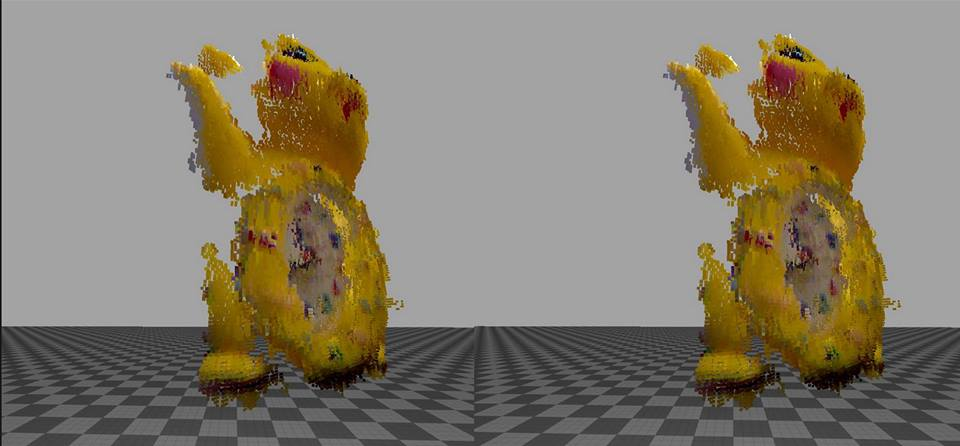
\includegraphics[width=0.9\textwidth]{pika4}
    \caption{Pikachu Render}
    \label{fig:awesome_image}
  \end{subfigure}
  \begin{subfigure}[b]{0.45\textwidth}
    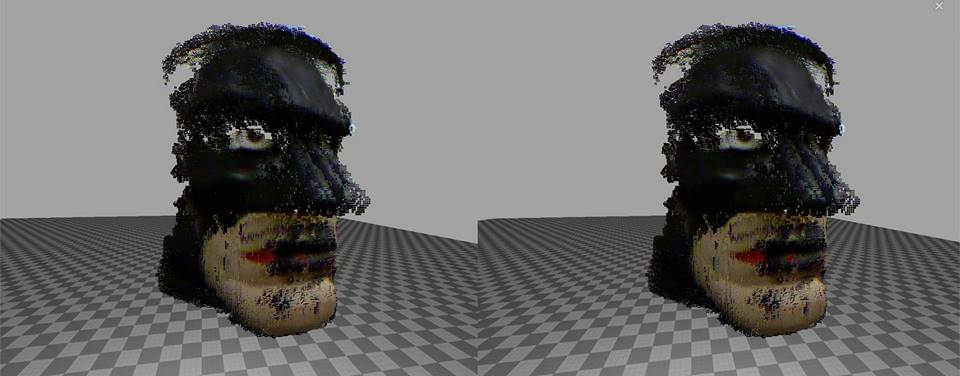
\includegraphics[width=0.8\textwidth]{batman}
    \caption{Batman Render}
    \label{fig:awesome_image}
  \end{subfigure}
\end{figure}

We initially set two goals for this section of the project. We primarily wanted
to view one of our 3D scans in the web app we created for Cardboard. We set as
an additional goal the ability to view the object from multiple viewpoints. We
were able to complete the first goal by being able to view our own PLY files in
the space, as demonstrated in the image. 

However, we were not able to complete the rotation segment of our goals.
Originally when we were using OBJ files, this process was not difficult, as we
could rotate the entire object together. We were even able to rotate the
object using the device's pitch and yaw to integrate the virtual reality space
better. However, when we converted to PLY, this became much more difficult as
we would be rotating the individual points. Thus, we did not continue to
rotate the object and instead allowed the user to rotate in the scene, where
the object was stationary. At any rate, this proved an insignificant
hindrance, as our 3D reconstruction only extended to the front 180 degrees of
the object, and therefore the ability to see the back of the object became
unnecessary.


\end{document}

